% document based on the VU Beta / BSc Thesis template

\documentclass[11pt]{article}
\usepackage{graphicx}
\usepackage{hyperref}

      \textwidth 15cm
      \textheight 22cm
      \parindent 10pt
      \oddsidemargin 0.85cm
      \evensidemargin 0.37cm

%
\usepackage{xcolor}  % Colored text etc.
%
\definecolor{OwnAzure}{HTML}{336699}
\definecolor{OwnCerulean}{HTML}{CAE2FE}
\definecolor{OwnOliveGreen}{HTML}{556B2F}
%
\usepackage[colorinlistoftodos,prependcaption,textsize=tiny]{todonotes}% Add ,disable to the options, to hide the comments
%
%
\usepackage{xargs}                      % Use more than one optional parameter in a new commands
%
\newcommand{\todojacob}[1]{\todo[inline, color=OwnAzure!40]{Jacob: #1}}
\newcommand{\todoalexandru}[1]{\todo[inline, color=orange!40]{Alexandru: #1}}

\newcommand{\thoughts}[1]{\todo[inline, color=OwnOliveGreen!40]{Question: #1}}
\graphicspath{ {./images/} }
\begin{document}

\thispagestyle{empty}
\newcommand{\opendc}{OpenDC}

\begin{center}

Vrije Universiteit Amsterdam

\vspace{1mm}


\includegraphics[height=28mm]{vu-griffioen-white.pdf}

\includegraphics[height=28mm]{atLarge.jpg}

\vspace{1.5cm}

{\Large Bachelor Thesis}

\vspace*{1.5cm}

\rule{.9\linewidth}{.6pt}\\[0.4cm]
{\huge \bfseries Title of the Research Project\par}
{\huge \bfseries Comes Here\par}\vspace{0.4cm}
\rule{.9\linewidth}{.6pt}\\[1.5cm]

\vspace*{2mm}

{\Large
\begin{tabular}{l}
{\bf Author:} ~~Jacob Burley ~~~~ (2599965)
\end{tabular}
}

\vspace*{1.5cm}

\begin{tabular}{ll}
{\it 1st supervisor:}   & ~~dr. Alexandru Iosup \\
{\it 2nd reader:}       & ~~Laurens Versluis
\end{tabular}

\vspace*{2cm}

\textit{A thesis submitted in fulfillment of the requirements for\\ the VU Bachelor of Science degree in Computer Science}

\vspace*{1cm}

\today\\[4cm] % Date

\end{center}

\newpage

\tableofcontents
\newpage
\listoffigures
\listoftables
\newpage


\section*{Abstract}
Will be written last.
\newpage

\section{Introduction} \label{sec:introduction}
	
	\subsection{\opendc{}}
		With the rapid expansion in the use of cloud services by both consumers and businesses \cite{Kushida2015}\cite{mokhtar2013}, the data centers that house these services must also grow. 
		While many may not see the cloud in its physical manifestation, cloud services are provided by servers, and servers are typically stored in data centers. 
		The configuration of such servers varies drastically, depending on the intended workload. 
		Relational databases, for example, can have large memory requirements. 
		Likewise, file servers may not need a particularly powerful CPU, but do require a lot of disks, and perhaps even a network card with higher throughput.

		When architecting data centers, many stakeholders must come together and agree on the various specifications of the data center, each with their own unique set of requirements. 
		System architects will then begin to design a system that meets these requirements. 
		However, such projects also have constraints. 
		Designing a data center isn't as easy as buying servers that meet the requirements of the stakeholders and putting them into use. 
		Constraints such as budget or physical space often influence design decisions, with smaller data centers perhaps comprising of higher-density compute nodes. 
		Designing data centers is often a complex problem, for which no validated analytical models exist. 
		Despite some academic institutions often being forthcoming with the technologies used in their data centers, there is no one-size-fits-all approach for data center design, making it hard to determine what hardware you need for a given workload.
		
		We focus in this work on \opendc{}, an open-source Discrete Event Simulator used to simulate the performance of workloads on massive computer systems. 
		Its purpose is to assist in performance testing of data centers designed by users, with the intention that the information gained can be factored in when these systems are being designed. 
		\opendc{} simulates workloads using traces from the Grid Workload Archive \cite{Iosup2008}, which are provided by participants who contribute to the archive. 
		These traces provide metadata about the scheduling requirements of jobs frequently sent to data centers, such as CPU usage throughout a job. 
		Using this information, \opendc{} can simulate the speed with which a workload will complete, as well as resource usage throughout the workload. 
		These simulations can assist businesses and educational institutions in highlighting and addressing performance concerns in their next-generation environments before any hardware has even been purchased.
	
	\subsection{Problem}
		In its current state, \opendc{} can be used to simulate user-specified workloads on user-designed systems. 
		Users must specify each individual component used, and build out an entire system. 
		This requires a high level of technical understanding, and relies solely on the user's knowledge of the intended workload when component choices are made. 
		In this way, the reasoning behind component choices has to be expressed by the individual, rather than \opendc{} itself.  

		With the implementation of prefabricated components (prefabs), hardware choices can be made by \opendc{}, with the user simply specifying which workload(s) they want to run.
		Prefabs would be then be complete collections of components intended for a specific workload, so that all that would be needed to design a datacenter was knowledge of its intended purpose.
		A user could then drag and drop the components required for certain services into their datacenter design, which would provide at least a starting point to build off of, allowing for accelerated prototyping.

		Because workloads scale, prefabs can scale with them.
		Prefabs could consist of a single server, but could also scale up to a rack full of servers, or even a room full of equipment.
		This approach would enable users reliant on homogenous hardware configurations to save their standard configurations as prefabs, further saving time when they need to add more of the same kind of node in new designs.
	
	\subsection{Research Questions}
		In this thesis, we aim to improve the ease of use of \opendc{}, while also implementing a new, easily-expandable representation of datacenter hardware that allows for accurate technical descriptions of hardware. 
		In doing so, we answer the following three questions:
		\todojacob{Reword the RQs to flow a little better and be a little clearer.}
		\begin{itemize}
			\item [\textbf{RQ1:}] How do we design a prefab abstraction that accurately describes important technical and composable features?
			\item [\textbf{RQ2:}] How to further allow operations, extensions, and the sharing of data?
			\item [\textbf{RQ1:}] How can we test and validate the use of prefabs to define hyperconverged/HPC datacenter topologies?
		\end{itemize}
	
	\subsection{Approach}
		The approach begins with understanding the shortcomings of the current implementation of topologies in \opendc{}.
		Next, we seek to understand the components that are important to represent in the datastructure, as well as identify components we no longer need to represent.
		From here, we examine a variety of common methods of representing data, and assess their suitability towards our desired way of representing datacenter hardware.
		Following on from this, we present a datastructure design, as well as the decisions made during the design process, and validate it through a prototyping stage.
		Lastly, we implement the datastructure design and accompanying technologies into \opendc{}.
	
	\subsection{Main Contribution of the Work}
		This thesis pioneers a new approach to representing datacenter hardware within a datacenter simulator.
		The main contributions of this thesis are:
		\begin{enumerate}
			\item A design for a datastructure that can be used to store datacenter hardware representations that is also easily usable and expandable, as well as an evaluation of said design in terms of the suitability of the datastructure for purpose.
			\item An implementation of this design into the main codebase of \opendc{}, as well as an evaluation of this design comparing usability to the previous version of \opendc{}.
		\end{enumerate}
	
	\subsection{Thesis Outline}
		The first chapter provides a short introduction to the current state of datacenter design, as well as the current state of OpenDC. 
		Chapter 2 provides more background on how modularity is currently used in computing, both in datacenters and in fields such as software engineering. 
		In Chapters 3 and 4, we design a prefab datastructure, reason about the choices that have been made during the design process, and touch on the process of implementing our chosen datastructure into the \opendc{} codebase.
		Chapter 5 provides an assessment of the suitability of the datastructure and technologies we chose, now that they have been implemented in \opendc{}.
		Finally, we discuss both the conclusion and future of this endeavour in Chapter 6.
	

	

\newpage

\section{Background} \label{sec:background}

	\subsection{A Topological View of Datacenters}
		In general, individuals working with datacenters think about their datacenter in terms of its topology. 
		Often, this takes the form of a network topology \cite{Couto2012}, where a spanning tree is built from all of the participating nodes. 
		\begin{figure}[htb]
			\centering
			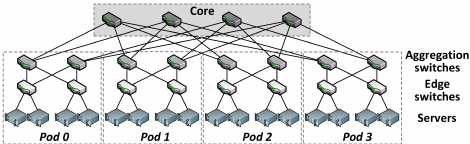
\includegraphics[width=8cm]{couto2012/Fat-tree-with-4-port-switches-n-4.png}
			\caption[A conventional network-focussed datacenter topology]{A conventional network-focussed datacenter topology \cite{Couto2012}}
		\end{figure}
		For \opendc{}, however, it is important to consider the parent-child relationships between the hardware components themselves. 
		For example, we can consider a chassis residing within a given rack to be a child of that rack, with good datacenter practice requiring that an in-use chassis is not kept outside of a rack.
		By defining these inter-component relationships, we can build our own spanning tree model, which allows us to easily manipulate parent objects and all of their children by simply moving the parent object elsewhere in the tree, reshaping our topology.
	
	\subsection{Modularity in Computing}
		In software architecture, it is becoming increasingly common to rely on frameworks and libraries written by others in the software engineering community. 

		This process would be akin to the modularity already seen in software engineering, where a programmer may import a library (often written by someone else) to enable certain functionality in their program. 
		The programmer often only uses one or two functions from this library, and does not necessarily understand how these functions work (nor do they need to).
		It is usually not necessary to understand the full workings of such a library, as the benefit comes from its utility in meeting certain requirements. 
		We can view these software modules as prefabricated software, which an individual may add into their project with ease. 
		Such a module may be added manually, by copying the relevant source files into the project, or may be added by means of a package manager.
		\verb|npm| is a package manager for \verb|node.js| that seeks to make installing dependencies much easier for developers \cite{Wittern2016}.
		For open-source projects a developer can include a file listing all of the external packages they used in their project, as well as the specific versions of each of these packages, so that another individual can easily run the authors software on their own machine.
		\verb|npm| also enables package authors to publish their packages in an online registry, so that other developers may download and use them.
		It follows, then, that it would be helpful to be able to describe datacenter hardware, and share these descriptions, in such a way. 
		With the advent of PaaS and particularly SaaS offerings from major cloud providers, developers can implement entire layers of their software stack with just a few clicks. 
		These layers still run in virtual machines, but the developer does not need to concern themselves too much with building or maintain the hardware or operating system.
		This concept is already offered by some cloud providers: DigitalOcean is a Virtual Private Server (VPS) provider that harnesses a "marketplace" of pre-configured VPS templates (known as "1-Click Apps") in order to simplify use of the platform \cite{DigitalOcean2020}. 
		Customers can then easily add a pre-configured VPS to their environment, without having to worry about operating system installation, configuration, or maintenance. 
		Templates provided through the platform are typically created by the vendors of the software used in each template, and are thus of high quality and suitability for the application.
	
	\subsection{The Goal of Prefabs}
		Users of \opendc{} would benefit from prefabs in much the same way, only having to focus on which services they want to run in their datacenter.
		Large datacenter providers using \opendc{} may also see a benefit. 
		Cloud service providers who provide IaaS services typically use homogenous hardware configurations, with different configurations for each performance tier. 
		With prefabs, it would be straightforward to create a prefab that is representative of a given performance tier, and then clone it when performing capacity planning during periods of growth.
	
	\subsection{Formats for Specifying Prefabs}
		When considering a new format for representing our new datastructure, we must first identify the important qualities that a suitable format must have. 
		A functional requirement for the format is that it must support nested objects. 

		The current \opendc{} database uses 35 SQL tables, 20 of which are used to store topologies.
		As a result, adding hardware items to the database requires a complex set of queries, with deletions and modifications requiring additional queries.
		In order to reduce the complexity associated with \opendc{}, we seek a storage format that allows us to store entire prefabs (as well as topologies) within a single object.
		The advantage of such an approach is that the database then only has to support the adding, updating and deleting of prefabs.

		In order to further the goal of simplifying working with \opendc{}, we also transition the storage database away from SQL, towards a noSQL design.
		We choose MongoDB as a document storage solution due to its ease of use, as well as its flexibility.
		MongoDB supports the insertion of JavaScript Object Notation (JSON) objects.
		JSON is an expressive, industry-standard object storage format that is widely used in web-based applications.
		It is both human-readable, and supports nested object hierarchies.
		As a result, it meets our functional requirements.

		We consider several formats for representing our datastructure.
		\todojacob{Rewrite in progress}
		First, we consider \textit{YAML Ain't Markup Language} (YAML) as our document format.
		YAML is both human as well as machine readable, and supports nested object hierarchies.
		However, we find that YAML is not suitably human-readable.
		It relies on indentation for distinguishing levels of hierarchy, with no clear boundaries delimiting separate objects.

		\textit{Extensible Markup Language} (XML) is a common language for storing and representing documents that is used in many web applications.
		It is both human and machine readable by design, and is well suited to nested object hierarchies, making it a strong contender to be used to store prefabs.
		However, XML requires parsing.
		The current \opendc{} frontend is written in \verb|ReactJS|, which does not natively support parsing XML without the use of an external library.
		As we prefer not to add additional dependencies to \opendc{}, we do not find XML to be a suitable choice as a document format.
	
	\subsection{Domain-Specific Prefabs}
		Datacenters have many intended uses, depending on the intended domain of the datacenter.
		The design of datacenters, as well as the component choices made during the design process, varies significantly depending on the intended use.
		Some datacenter owners choose to focus on a hyperconverged infrastructure, where a many-core approach is taken to provide sufficient resources to virtualize much of the environment.
		In such a scenario, hardware is not chosen based on the suitability for one application, but to support the flexibility to be able to run any application in virtual machines.
		This is especially common in industry, with the intention of reducing downtime.
		Virtual machines can be migrated between physical hosts while still running when hardware maintenance is required.
		It is also possible to add resources to a virtual machine without power loss, dynamically scaling them to jobs.

		Conversely, other datacenter owners may focus on High-Performance Computing (HPC).
		These datacenters are designed differently, with a high number of nodes running a baremetal operating system.
		The configuration of these nodes varies, depending on the intended use of the node.
		Nodes are then categorized into performance tiers based on their intended use.
		Performance tiers are then chosen by customers depending on the kind of workload they want to run - for example, GPUs may be installed in the nodes in tiers intended for Machine Learning workloads.

		Prefabs specific to certain domains can be represented in \opendc{}, with different performance tiers included within each domain.
		In this way, users can easily build massive, homogenous systems by selecting the node specific to their performance target, and using it as a starting point.


\section{A Design for a Representation of Data Center Hardware}

	\subsection{A model for datacenter representation}
		In this research, we provide a model for representing datacenter hardware. 
		This model is not the first of its kind: Andreadis et al created a model for datacenter hardware in order to model scheduling in \opendc{} \cite{Andreadis2018}. 
		Our model, however, offers more detail, storing more characteristics of the hardware within.
		When designing the model, it is important to consider that a large part of its purpose is to increase usability of \opendc{}. 
		As a result, we choose to represent lots of hardware characteristics that are not used by the simulator, but provide useful information to the user. 
		Brands of hardware are not necessary in order to simulate workloads, but they are useful when a user is making design decisions, or presenting their design to a wider audience.
		Conversely, performance metrics such as how many millions of instructions per second (MIPS) a processor can execute are of utmost importance to the simulator when extrapolating performance numbers, but are generally meaningless to stakeholders without a technology background.
	
	\subsection{A definition and design of a datastructure for storing prefabs}
		\todojacob{Rewrite}
		In order to store our datacenter hardware representation within \opendc{}, we define a datastructure to represent the datacenter hardware. 
		This datastructure aims to be simple to understand, as well as easily expandable in order to represent hardware configurations that we do not focus on in this research (i.e. blade servers, or other chassis that may contain multiple/unconventional motherboards). 
		For this reason, we choose to use JavaScript Object Notation (JSON) to store our datastructure. 
		This supports our goals of ease of use and expandibility, as JSON is a human-readable industry-standard object storage format that can be extended to represent a variety of objects.
		\todojacob{Reword the above line}



	\subsection{Designing ways to create and interact with prefabs}
		When determining interactions we prefabs, we must define a set of operations that is sufficient to execute the intended purpose of prefabs.
		
\section{Implementation of a Prototype}

	\subsection{Why prototype?}
		Prototyping is an important part of our design process for implementing the new topologies in \opendc{}.
		The design proposal requires the implementation of certain new technologies (such as MongoDB) which we are unfamiliar with.
		As a result, prototyping provides us with a way of becoming familiar with these new technologies, as well as assessing their suitability, before we begin the process of implementing them into the existing \opendc{} codebase.
		We also can create prototypes of the datastructure, as well as the corresponding interactions with it, and assess the suitability of the datastructure with regards to the interactions we require it to be capable of handling.
	
	\subsection{Creating a prototype}
		The two main learning outcomes of prototyping are to explore how we can best implement and interact with MongoDB, and to iteratively improve our datastructure design.
		As a result, the prototype consists of three components: a MongoDB instance, a Python module that interfaced with the database, and a second Python application to serve as a rudimentary frontend. 
		This configuration has been chosen to be relatively close to how \opendc{} already implements its database connections, which also uses a Python module to abstract away most database interactions.

		MongoDB has been chosen in order to easily facilitate the storage of our JSON objects.
		MongoDB stores documents in a JSON-like format internally, and has strong library support for inserting, modifying and exporting said documents, making it relatively straightforward to re-implement our database connection.
	
	\subsection{The process of implementing the prototype}

	\subsection{Validating Prototypes}

	\subsection{Lessons learned}
		During prototyping, we learnt many things that influenced the decisions we made during the implementation phase.
		We also learnt a lot about the differences between MongoDB and SQL, which allowed us to improve how we implement this new database technology throughout \opendc{}.

\section{Evaluation of Design \& Implementation}


\section{Conclusion} \label{sec:conclusion}

\section{Future Work}
	\todojacob{Adding this here for now, will likely merge future work into conclusion at a later date.}
	Looking forward, it would be beneficial for \opendc{} to simulate user-specified workloads on systems designed by \opendc{} itself. 
	\opendc{} would be able to leverage a large database of performance data to make component choices based on the workload specified by the user. 
	In this way, the system would be designed for the best objective performance at the specified workload, potentially adherent to specified constraints such as financial or power budget.


\newpage
% For more on bibliography styles, see 
% https://www.overleaf.com/learn/latex/Bibtex_bibliography_styles
\bibliographystyle{abbrv}
\bibliography{main}


\end{document}
% \end{document}



